% !TEX root = poster.tex
\node [mybox,anchor=north west, font=\fontsize{\fntszL}{\fntszL}\selectfont]
at (\ideaPos) (boxIdea){%
\begin{minipage}{\bxszA}

\bigskip
\bigskip
\bigskip
\textbf{\centerline{Embed uncertainty within the model}}

\scalebox{0.75}{
\centerline{
\hspace*{10cm}
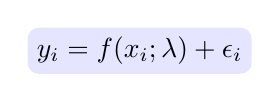
\begin{tikzpicture} \node [rounded corners,fill=blue!10] {
$y_i=f(x_i;\lambda)+\epsilon_i$
};
\end{tikzpicture}
\hspace*{2cm}
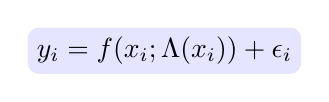
\begin{tikzpicture} \node [rounded corners,fill=blue!10] {
$y_i=f(x_i;\Lambda(x_i))+\epsilon_i$
};
\end{tikzpicture}
\hspace*{2cm}
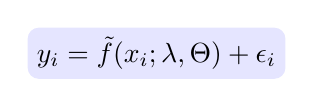
\begin{tikzpicture} \node [rounded corners,fill=blue!10] {
$y_i=\tilde{f}(x_i;\lambda,\Theta)+\epsilon_i$
};
\end{tikzpicture}
}
}

\emph{\hspace*{3.3cm}Black-box \hspace*{2.9cm} Random field \hspace*{2.3cm} Extra `physics'}

\begin{itemize}
\item Embed model error in specific submodel phenomenology
\item Allows targeted model error placement
\item Preserves model structure and physical constraints
\item Disambiguate model and data errors

\end{itemize}


\end{minipage}
};
\node[fancytitle, right=10pt, font=\fontsize{\fntszL}{\fntszL}\selectfont]
at (boxIdea.north west) {\bf Idea: Embedded Model Error};

